% Options for packages loaded elsewhere
\PassOptionsToPackage{unicode}{hyperref}
\PassOptionsToPackage{hyphens}{url}
\PassOptionsToPackage{dvipsnames,svgnames,x11names}{xcolor}
%
\documentclass[
  11pt,
  letterpaper,
  oneside]{book}

\usepackage{amsmath,amssymb}
\usepackage{iftex}
\ifPDFTeX
  \usepackage[T1]{fontenc}
  \usepackage[utf8]{inputenc}
  \usepackage{textcomp} % provide euro and other symbols
\else % if luatex or xetex
  \usepackage{unicode-math}
  \defaultfontfeatures{Scale=MatchLowercase}
  \defaultfontfeatures[\rmfamily]{Ligatures=TeX,Scale=1}
\fi
\usepackage{lmodern}
\ifPDFTeX\else  
    % xetex/luatex font selection
\fi
% Use upquote if available, for straight quotes in verbatim environments
\IfFileExists{upquote.sty}{\usepackage{upquote}}{}
\IfFileExists{microtype.sty}{% use microtype if available
  \usepackage[]{microtype}
  \UseMicrotypeSet[protrusion]{basicmath} % disable protrusion for tt fonts
}{}
\makeatletter
\@ifundefined{KOMAClassName}{% if non-KOMA class
  \IfFileExists{parskip.sty}{%
    \usepackage{parskip}
  }{% else
    \setlength{\parindent}{0pt}
    \setlength{\parskip}{6pt plus 2pt minus 1pt}}
}{% if KOMA class
  \KOMAoptions{parskip=half}}
\makeatother
\usepackage{xcolor}
\usepackage[left=1in,right=1in,top=1in,bottom=1in]{geometry}
\setlength{\emergencystretch}{3em} % prevent overfull lines
\setcounter{secnumdepth}{5}
% Make \paragraph and \subparagraph free-standing
\ifx\paragraph\undefined\else
  \let\oldparagraph\paragraph
  \renewcommand{\paragraph}[1]{\oldparagraph{#1}\mbox{}}
\fi
\ifx\subparagraph\undefined\else
  \let\oldsubparagraph\subparagraph
  \renewcommand{\subparagraph}[1]{\oldsubparagraph{#1}\mbox{}}
\fi


\providecommand{\tightlist}{%
  \setlength{\itemsep}{0pt}\setlength{\parskip}{0pt}}\usepackage{longtable,booktabs,array}
\usepackage{calc} % for calculating minipage widths
% Correct order of tables after \paragraph or \subparagraph
\usepackage{etoolbox}
\makeatletter
\patchcmd\longtable{\par}{\if@noskipsec\mbox{}\fi\par}{}{}
\makeatother
% Allow footnotes in longtable head/foot
\IfFileExists{footnotehyper.sty}{\usepackage{footnotehyper}}{\usepackage{footnote}}
\makesavenoteenv{longtable}
\usepackage{graphicx}
\makeatletter
\def\maxwidth{\ifdim\Gin@nat@width>\linewidth\linewidth\else\Gin@nat@width\fi}
\def\maxheight{\ifdim\Gin@nat@height>\textheight\textheight\else\Gin@nat@height\fi}
\makeatother
% Scale images if necessary, so that they will not overflow the page
% margins by default, and it is still possible to overwrite the defaults
% using explicit options in \includegraphics[width, height, ...]{}
\setkeys{Gin}{width=\maxwidth,height=\maxheight,keepaspectratio}
% Set default figure placement to htbp
\makeatletter
\def\fps@figure{htbp}
\makeatother
\newlength{\cslhangindent}
\setlength{\cslhangindent}{1.5em}
\newlength{\csllabelwidth}
\setlength{\csllabelwidth}{3em}
\newlength{\cslentryspacingunit} % times entry-spacing
\setlength{\cslentryspacingunit}{\parskip}
\newenvironment{CSLReferences}[2] % #1 hanging-ident, #2 entry spacing
 {% don't indent paragraphs
  \setlength{\parindent}{0pt}
  % turn on hanging indent if param 1 is 1
  \ifodd #1
  \let\oldpar\par
  \def\par{\hangindent=\cslhangindent\oldpar}
  \fi
  % set entry spacing
  \setlength{\parskip}{#2\cslentryspacingunit}
 }%
 {}
\usepackage{calc}
\newcommand{\CSLBlock}[1]{#1\hfill\break}
\newcommand{\CSLLeftMargin}[1]{\parbox[t]{\csllabelwidth}{#1}}
\newcommand{\CSLRightInline}[1]{\parbox[t]{\linewidth - \csllabelwidth}{#1}\break}
\newcommand{\CSLIndent}[1]{\hspace{\cslhangindent}#1}

% section formatting
\usepackage{fancyhdr}
\renewcommand{\chaptername}{Section}
\pagestyle{plain}
\makeatletter
\makeatother
\makeatletter
\@ifpackageloaded{bookmark}{}{\usepackage{bookmark}}
\makeatother
\makeatletter
\@ifpackageloaded{caption}{}{\usepackage{caption}}
\AtBeginDocument{%
\ifdefined\contentsname
  \renewcommand*\contentsname{Table of contents}
\else
  \newcommand\contentsname{Table of contents}
\fi
\ifdefined\listfigurename
  \renewcommand*\listfigurename{List of Figures}
\else
  \newcommand\listfigurename{List of Figures}
\fi
\ifdefined\listtablename
  \renewcommand*\listtablename{List of Tables}
\else
  \newcommand\listtablename{List of Tables}
\fi
\ifdefined\figurename
  \renewcommand*\figurename{Figure}
\else
  \newcommand\figurename{Figure}
\fi
\ifdefined\tablename
  \renewcommand*\tablename{Table}
\else
  \newcommand\tablename{Table}
\fi
}
\@ifpackageloaded{float}{}{\usepackage{float}}
\floatstyle{ruled}
\@ifundefined{c@chapter}{\newfloat{codelisting}{h}{lop}}{\newfloat{codelisting}{h}{lop}[chapter]}
\floatname{codelisting}{Listing}
\newcommand*\listoflistings{\listof{codelisting}{List of Listings}}
\makeatother
\makeatletter
\@ifpackageloaded{caption}{}{\usepackage{caption}}
\@ifpackageloaded{subcaption}{}{\usepackage{subcaption}}
\makeatother
\makeatletter
\@ifpackageloaded{tcolorbox}{}{\usepackage[skins,breakable]{tcolorbox}}
\makeatother
\makeatletter
\@ifundefined{shadecolor}{\definecolor{shadecolor}{HTML}{f2f2f2}}
\makeatother
\makeatletter
\@ifundefined{codebgcolor}{\definecolor{codebgcolor}{HTML}{f2f2f2}}
\makeatother
\makeatletter
\makeatother
\ifLuaTeX
  \usepackage{selnolig}  % disable illegal ligatures
\fi
\IfFileExists{bookmark.sty}{\usepackage{bookmark}}{\usepackage{hyperref}}
\IfFileExists{xurl.sty}{\usepackage{xurl}}{} % add URL line breaks if available
\urlstyle{same} % disable monospaced font for URLs
\hypersetup{
  pdftitle={REU Research Report},
  pdfauthor={Olivia Davis and Gaoussou Toure},
  colorlinks=true,
  linkcolor={Maroon},
  filecolor={Maroon},
  citecolor={Blue},
  urlcolor={Blue},
  pdfcreator={LaTeX via pandoc}}

\title{REU Research Report}
\author{Olivia Davis and Gaoussou Toure}
\date{2023-06-20}

\begin{document}
\frontmatter
\maketitle
\ifdefined\Shaded\renewenvironment{Shaded}{\begin{tcolorbox}[boxrule=0pt, frame hidden, colback={codebgcolor}, borderline west={3pt}{0pt}{shadecolor}, enhanced, breakable, sharp corners]}{\end{tcolorbox}}\fi

\renewcommand*\contentsname{Contents}
{
\hypersetup{linkcolor=}
\setcounter{tocdepth}{4}
\tableofcontents
}
\mainmatter
\bookmarksetup{startatroot}

\hypertarget{introduction}{%
\chapter*{Introduction}\label{introduction}}
\addcontentsline{toc}{chapter}{Introduction}

\markboth{Introduction}{Introduction}

\bookmarksetup{startatroot}

\hypertarget{week-jun-11---jun-17}{%
\chapter{Week Jun 11 - Jun 17}\label{week-jun-11---jun-17}}

\hypertarget{background}{%
\section{Background}\label{background}}

\begin{itemize}
\tightlist
\item
  Phylogenetic trees

  \begin{itemize}
  \tightlist
  \item
    Depict the lines of evolutionary descent of different species or
    genes from a common ancestor
  \end{itemize}
\item
  Orthlogs and Paralogs

  \begin{itemize}
  \tightlist
  \item
    Orthologs are homologous genes in different species that diverged
    from a single ancestral gene after a speciation event
  \item
    Paralogs are homologous genes that originate from the duplication of
    an ancestral gene
  \end{itemize}
\item
  Newick Format

  \begin{itemize}
  \tightlist
  \item
    A way to encode phylogenetic trees
  \item
    An example is ``(A, (B, C));'', where A is the root and B and C are
    the two children.
  \end{itemize}
\end{itemize}

\hypertarget{methods}{%
\section{Methods}\label{methods}}

\begin{itemize}
\tightlist
\item
  Generate tree with dendropy
\item
  Visualize tree to confirm structure
\item
  Start at leaves a keep track of the genes we've come across and the
  species we've come across as we traverse up the tree by storing them
  in sets.
\item
  Also label relationships (orthologous or paralogous) as you compare
  children

  \begin{itemize}
  \tightlist
  \item
    If there is no shared taxons between the sets of the children, then
    we assume there is speciation event so we label paralogous
  \item
    If there is no shared genes between the sets of the children, then
    we assume there is a duplication event so we label paralogous
  \item
    No current handle for if both are true (see discussion below)
  \item
    If neither are true, no changes occured (we shouldn't see this, that
    would be a node splitting into two exact children (e.g.~(man-a,
    man-a))).
  \end{itemize}
\end{itemize}

\hypertarget{results}{%
\section{Results}\label{results}}

\begin{figure}

{\centering 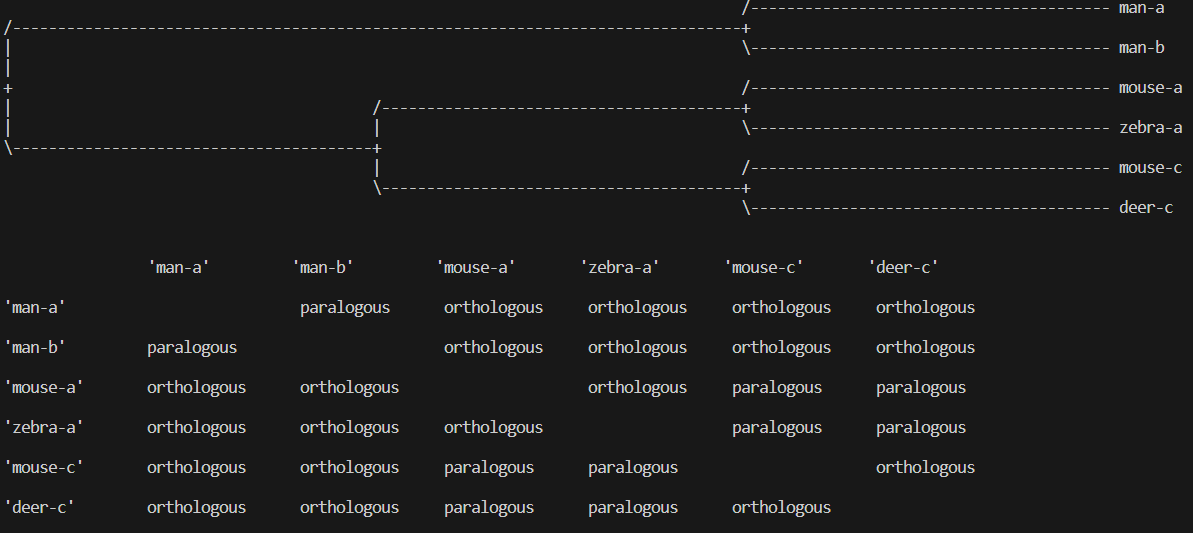
\includegraphics{./figures/Week1LabelingResult.PNG}

}

\caption{An example tree with a matrix of relationships between taxons.}

\end{figure}

\hypertarget{discussion}{%
\section{Discussion}\label{discussion}}

While working through a simple way to label the tree, we follow certain
assumptions that simplify the process. We need to know what kind of
cases we are working with and what a given tree would realistically look
like.

The above labelling only works for trees that always have a duplication
or speciation event and experience no gene loss. Further, we assume that
each of these events lead to unique taxons/gene ids. Our question for
this is whether a speciation (or duplication) event can lead to a
species (or geneid) we've seen before. For example, the tree below:

\begin{figure}

{\centering 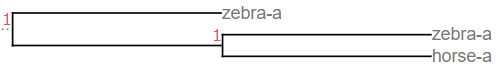
\includegraphics{./figures/RepeatSpecExample.PNG}

}

\caption{A tree with two speciations, resulting in two zebra species}

\end{figure}

Where we have the first speciation event split into the ``zebra-a'' and
``horse-a'' branches and then the horse branch splits into ``horse-a''
and ``zebra-a''. (The current assumption is that this is not possible).

Another case we need more context to cover is whether we can see a node
with children that differ in both the species and geneid such as,

\begin{figure}

{\centering 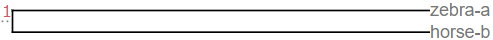
\includegraphics{./figures/AmbigousExample.PNG}

}

\caption{A tree with gene loss, making the paralogous/orthologous
relationship unclear.}

\end{figure}

Without more context (either from possible extra parameters or
comparison to other trees), we cannot confidently label the taxons as
orthologs or paralogs. In the two simplest cases, the above tree could
have resulted from duplication then speciation, or vice versa, with
there being gene loss of the ``zebra-b'' and ``horse-a'' taxons. Based
on which event occured first, the relationship changes.

Another point of discussion is inparalogs and outparalogs. Since those
relationships are relative to a certain event, is the user specifiying
what event to compare the relationships to?

As for the tool itself, we'd like to know what customizations might be
helpful. One thing we plan on adding is to change what the separator is
between the species and gene id. The default right now is ``-''. We also
have the display as a matrix, but this may be unsuitable for very large
trees. Some ideas are to output a file (text, cvs, etc.). We also store
the relationships in a nested dictionary, so it is easy to look up
specific relationships in constant time.

\bookmarksetup{startatroot}

\hypertarget{references}{%
\chapter*{References}\label{references}}
\addcontentsline{toc}{chapter}{References}

\markboth{References}{References}

\hypertarget{refs}{}
\begin{CSLReferences}{0}{0}
\end{CSLReferences}


\backmatter

\end{document}
